\documentclass{standalone}
\usepackage{pgfplots}
\pgfplotsset{compat=newest}
\begin{document}
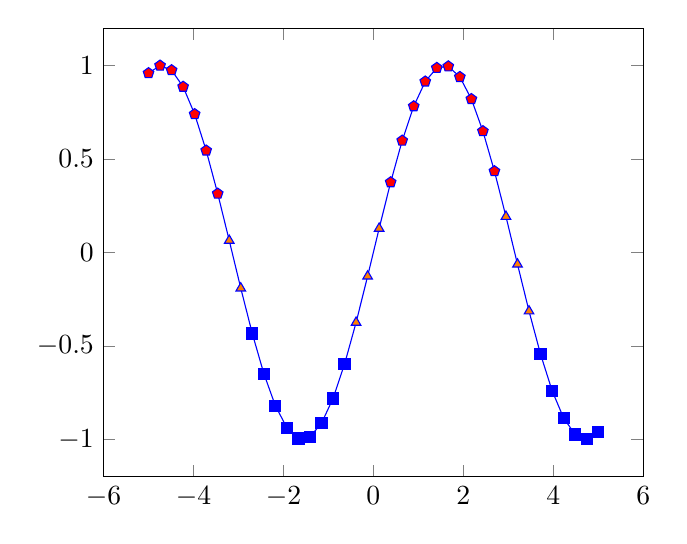
\begin{tikzpicture}
% Low-Level scatter plot interface Example: 
% use three different marker classes 
% 0% - 30%   : first class
% 30% - 60%  : second class
% 60% - 100% : third class
\begin{axis}[
scatter/@pre marker code/.code={%
   \ifdim\pgfplotspointmetatransformed pt<300pt
      \def\markopts{mark=square*,fill=blue}%
   \else
      \ifdim\pgfplotspointmetatransformed pt<600pt
         \def\markopts{mark=triangle*,fill=orange}%
      \else
         \def\markopts{mark=pentagon*,fill=red}%
      \fi
   \fi
   \expandafter\scope\expandafter[\markopts]
},%
scatter/@post marker code/.code={%
   \endscope
}]
\addplot+[scatter,scatter src=y,
	samples=40]
   {sin(deg(x))};
   
\end{axis}
\end{tikzpicture}
\end{document}
